\chapter{Methods}
\label{chapter:methods}

We now have all the building blocks needed to construct our method that implements projection mapping of textures by forcing the camera image to be a realization of the same texture as the desired appearance, instead of matching them pixel by pixel which is the usual approach (see section \ref{section:intro-key_idea} for more details on our key idea).

We will first present an overview of our projection mapping pipeline and then focus on its main components.

\section{Pipeline Overview}
\label{section:methods-pipeline_overview}

\begin{figure}[]
    \centering
    \def\svgwidth{\textwidth}
    \input{images/figures/03-pipeline.pdf_tex}
    \caption{{\color{red} TODO: the blue arrow thing is confusing. emphasize that \(p\) is the unknown!} An overview of our pipeline with \(y\) as input and \(p\) that minimizes eq. \ref{eq:projection_mapping-statistics} as output. The blue part of the diagram is essentially a texture synthesis pipeline by \citet{Gatys2015}. The green part (the rendering function) is our extension that enables projection mapping. Instead of computing a set of statistics \(f\) on the synthesized image \(p\) directly as \citet{Gatys2015} does (blue arrow), we first project \(p\) to obtain \(x(p)\) and only then compute \(f\). The red projector symbol shows how \(p\) is projected onto a glass ball in our scene and the white scissors symbol shows how the camera image is cropped because we only want to match a portion of the scene. The whole process is an optimization loop with \(p\) initialized to white noise and progressively refined until \(x(p)\) is a realization of the same texture as \(y\) is. Texture source: \citet{Pixar128}}
    \label{fig:methods_pipeline}
\end{figure}

Projection mapping is typically done with a projector-camera system (see fig. \ref{fig:intro_procam} for an example). However, we have decided to implement our system entirely as a software pipeline with simulated projector and camera for the following reasons:

\begin{itemize}
    \item A software implementation serves as necessary reference for future work. If something does not work in the controlled environment of a simulator, it will not work in the real world either
    \item Hardware systems come with challenges of its own, like signal-to-noise ratio, dynamic environment and time constraints. We want to focus on solving one challenge at a time, starting with projection quality
    \item Software pipelines are easier to modify and allow for rapid prototyping and experimentation
\end{itemize}

The goal of our pipeline is to minimize the expression in eq. \ref{eq:projection_mapping-statistics}. The main input is an image \(y\) which represents the desired appearance for our scene. Other inputs are the scene and projector which determine a rendering function \(x\) which creates a camera image \(x(p)\) out of a projector image \(p\). A projector image \(p\) which minimizes eq. \ref{eq:projection_mapping-statistics} is the output of the pipeline. See fig. \ref{fig:methods_pipeline} an illustration of how the pipeline works.

We build on top of a pipeline for texture synthesis used in \citet{Gatys2015} and extend it by the rendering function \(x\). The original synthesis pipeline is differentiable and relies on the gradient-based L-BFGS optimizer to synthesize a texture. Therefore, it is key that our \(x\) differentiable as well. This allows us to rely on L-BFGS to minimize eq. \ref{eq:projection_mapping-statistics}.

In section \ref{section:background-texture_synthesis}, we have reviewed several texture synthesis methods that could potentially be used in our method. We have decided to use \citet{Gatys2015} over a patch-based method such as \citet{Efros2001} for the following reasons:

\begin{itemize}
    \item It achieves good results for a large variety of textures
    \item It defines a texture model which can be (and has been, as we will discuss later) improved to achieve better results while keeping the rest of the pipeline fixed
    \item It is very easy to adapt for projection mapping and does not impose any restrictions on the rendering function. In fact, a gradient-free version of the pipeline could theoretically be run on a physical projector-camera system
    \item Using an optimizer to gradually improve the result allows us to obtain a reasonable result quickly and improve it if more time is available
\end{itemize}

We will now describe the two main components of our pipeline -- the rendering function \(x\) and the texture model which determines a set of statistics \(f(y)\) that fully describe a texture \(y\) -- in more detail.

\section{Rendering Function}
\label{section:methods-rendering_function}

The rendering function in our pipeline has the following form:

\begin{equation}
    \label{eq:rendering_function}
    x(p, \phi) = y  
\end{equation}

where \(p\) is the projector image, \(\phi\) are scene parameters, such as geometry, materials, projector and camera position and orientation and so on. \(y\) is the camera image whose statistics are matched against those of the input texture image (i.e. desired appearance). \(x\) needs to be differentiable because the statistics matching is done via gradient-based optimization.

\(x\) represents the act of projecting an image onto a scene and then capturing that projection. This is a fairly complex task, especially if the scene has arbitrary geometry, materials and external illumination. Luckily, in certain special scenarios, \(x\) can be very simple to formulate and fast to compute. We take advantage of this and use two different versions of \(x\) in our pipeline, a simple one to verify basic functionality and obtain reference results, and a general one to support arbitrary scenes.

\subsection{Simple Rendering Function}
\label{section:methods-rendering_function-simple}

Here is a scenario in which the light transport between the projector and the camera is easy to model:

\begin{itemize}
    \item The projector is pointed directly at a flat wall, with a right angle between its optical axis and the surface of the wall
    \item The surface of the wall is completely diffuse, meaning it looks matte and its appearance is not view-dependent
    \item The camera coincides with the projector
    \item We ignore light that is reflected from the wall into the rest of the scene and back into the camera
\end{itemize}

\begin{figure}[]
    \centering
    \def\svgwidth{0.6\textwidth}
    \input{images/figures/03-simple_scenario.pdf_tex}
    \caption{An illustration of the scenario modelled by the simple rendering function. The projector is pointed directly at the wall and coincides with the camera which allows for substantial simplification of the rendering process.}
    \label{fig:methods_simple_scenario}
\end{figure}

This scenario (see fig. \ref{fig:methods_simple_scenario} for an illustration) is not too unrealistic -- it is a reasonable approximation of projecting onto a textured wall in a living room where the camera is right next to the projector and thus the projector-camera correspondence is straightforward to recover (as mentioned in section \ref{section:background-projection_mapping-procams-radiometric_calibration}, inter-reflection is minimal in this case and thus a 1:1 correspondence between projector and camera pixels can be assumed). See figs. \ref{fig:intro_grossberg} and \ref{fig:intro_result_teaser} for examples where such a scenario can be used.

Let us now derive a rendering function that handles this simple scenario directly from the rendering equation:

\begin{align}
    L(x \rightarrow \mathbf{v}) &= \int_{\Omega(x)} L(x \leftarrow \mathbf{u}) f_r(x, \mathbf{u} \rightarrow \mathbf{v}) \cos \theta \mathrm{d}\mathbf{u} + E(x \rightarrow \mathbf{v}) \label{eq:simple_x_from_rendering_eq01} \\
    &= \int_{\Omega(x)} L(x \leftarrow \mathbf{u}) f_r(x, \mathbf{u} \rightarrow \mathbf{v}) \cos \theta \mathrm{d}\mathbf{u} \label{eq:simple_x_from_rendering_eq02} \\
    &= \int_{\Omega(x)} L(x \leftarrow \mathbf{u}) \rho \frac{\cos \theta}{\pi} \mathrm{d}\mathbf{u} \label{eq:simple_x_from_rendering_eq03} \\
    &= \int_{\Omega(x)} E(x \leftarrow \mathbf{u}) \rho \frac{\cos \theta}{\pi} \mathrm{d}\mathbf{u} \label{eq:simple_x_from_rendering_eq04} \\
    &\approx E(x \leftarrow \mathbf{-v}) \rho \frac{\cos \theta}{\pi r^2} \label{eq:simple_x_from_rendering_eq05}
\end{align}

Eq. \ref{eq:simple_x_from_rendering_eq01} is the rendering equation. We move to eq. \ref{eq:simple_x_from_rendering_eq02} by observing that our background is not an emitter in itself. Eq. \ref{eq:simple_x_from_rendering_eq03} is obtained by assigning the diffuse BRDF function \(\rho / \pi\) to the background surface. \(\rho\) is surface albedo which corresponds to the value of the background image at \(x\). \(\pi\) is a scaling constant needed to preserve energy in the scene. Eq. \ref{eq:simple_x_from_rendering_eq04} comes from our assumption that the only radiance that arrives at point \(x\) on the background comes from the projector. Finally, the integral can be approximated (eq. \ref{eq:simple_x_from_rendering_eq05}) by restricting the area we integrate over to the solid angle subtended by a projector pixel, assuming the integrand is constant over that area and setting \(u = v\). The area is inversely proportional to the square of the distance between the projector pixel and \(x\). Finally, we observe that \(E(x \leftarrow \mathbf{-v}) = p\) and \(\rho\) is the background image.

This leads us to the following straightforward and differentiable rendering function \(x\):

\begin{equation}
    \label{eq:rendering_function-simple}
    x(p, b) = c \cdot p \cdot b = y
\end{equation}

where \(p\) and \(y\) are again the projector and camera image, respectively, \(b\) is the background -- an image (texture) representing the surface of the wall -- and \(c\) is a constant that roughly accounts for \(\frac{\cos \theta}{\pi r^2}\). Here is where we perform the last simplification. \(r\) and \(\theta\) vary over the background and depend on how far the projector is from the background. However, we are only interested in simulating situations where the projector cannot be bright enough to compensate the projection with conventional methods but where it is still capable of compensating with our method. We thus set \(r\) ourselves to adjust the distance and the brightness of the projector according to our needs as part of a single constant \(c\). The variation of \(\cos \theta\) can be accounted for after the fact by darkening \(p\) towards the center. This means that we also have to assume that the minimum brightness of our projector is not limited by the scenario.

To summarize, the simple rendering function \(x\) can be very easily integrated into Gatys' synthesis pipeline and represents negligible computational overhead. This allows for rapid experimentation that yields reference results for a reasonable subset of projection scenarios. However, a more general solution for projection mapping on arbitrary 3D scenes is also needed. We cover it in the next section.

\subsection{General Scenario}
\label{section:methods-rendering_function-general}

A possible candidate for a general rendering function that computes camera images from projector image for arbitrary 3D scenes is simply a renderer such as PBRT (\citet{PBRT3e}) or Mitsuba (\citet{Mitsuba}). These renderers are programs that accept a scene configuration file as input and output an image of the scene as seen from the point of view of a virtual camera. For example, fig. \ref{fig:background_linear_lt} was created using Mitsuba. Renderers often implement a large variety of materials, camera effect, rendering equation solvers and other features that make them incredibly versatile. And indeed, they match the signature of our rendering function well:

\begin{equation}
    \label{eq:rendering_function-renderer}
    x(p, \textit{config}) = y
\end{equation}

where \(x\) is the renderer and \textit{config} represents the configuration file which also describes how the projector image \(p\) is used in the scene. However, renderers come with two main caveats:

\begin{itemize}
    \item They are generally not differentiable
    \item They require a complete description of scene geometry and materials which is rarely available in a projection mapping application
\end{itemize}

Both points are nowadays being addressed by differentiable renderers such as Mitsuba 2 (\citet{Mitsuba2}), but these systems are general-purpose and therefore too computationally heavy to be used in a texture synthesis pipeline. Instead, we use the fact that light transport in an arbitrary scene is linear and model our general rendering function \(x\) with a light transport matrix that was described in section \ref{section:background-projection_mapping-procams-inverse_lt}:

\begin{equation}
    \label{eq:rendering_function-lt_matrix}
    x(p, A) = c \cdot Ax = y
\end{equation}

where \(A\) is the light transport matrix (see \ref{eq:lt_matrix}) and \(p\) is supposed to be a vector representing the light sources in the scene. But this is exactly our projector image where each pixel corresponds to a light source that we can control separately. \(c\) is the same multiplier as in eq. \ref{eq:rendering_function-simple} whose purpose is to tune the overall brightness of the projector.

Multiplication by large matrices is differentiable, very fast on modern GPUs and the matrix size (and thus the computation time) depends only on the resolution of the projector and camera images, not on scene complexity. This makes them easy to use in a texture synthesis pipeline. However, the process of acquiring them is not entirely straightforward. We focus on it in the next section.

\subsubsection{Capturing the Light Transport Matrix}
\label{section:methods-rendering_function-general-lt_capture}

If a scene contains two lamps as light sources, then capturing a light transport matrix with respect to those lamps is nothing more than taking two photographs of the scene -- one for each lamp switched on separately. Our scene contains as many lamps as there are pixels in our projector image \(p\) (we can ignore other light sources because those are fixed). Taking a photograph for each of the projector pixels being switched on separately is practically impossible because of the signal-to-noise ratio of cameras -- no camera is able to capture such tiny signal as that coming from a single projector pixel.

If the goal is to capture an LT matrix of a real scene using a camera, there are other ways of doing it. Capturing one projector pixel at a time corresponds to capturing the canonical basis of the matrix (see fig. \ref{fig:background_lt_capture} for an illustration). As we saw in section \ref{section:background-projection_mapping-procams-inverse_lt}, different bases that comprise brighter pattern can be used as well. The fact that the matrix is often very sparse can also be used.

However, our projector-camera system is simulated fully in software which means that our scenes are virtual and we know precisely which geometry and materials they have. We can thus capture the canonical basis directly using a renderer whose floating-point arithmetic can handle tiny signals. We use Mitsuba to render camera images of our scene illuminated by each projector pixel separately and then assemble the images into the LT matrix \(A\). Note that the LT matrix capture is the main part of our pipeline that we simulate. The rest of the pipeline could work just as well with a different LT matrix \(A\) that would be captured from a real scene by a physical camera. See fig. {\color{red} TODO} for an illustration.

We now describe the capture process in more detail, focusing on how to configure Mitsuba for our purposes and how to work with the LT matrix. Specifically, we look at three topics:

\begin{itemize}
    \item How to implement a projector in Mitsuba?
    \item How to solve the rendering equation efficiently with only a single active projector pixel?
    \item How large is the light transport matrix and what are the implications?
\end{itemize}

\textbf{How to implement a projector in Mitsuba?} The Mitsuba renderer has very rudimentary projector functionality in the form of a spotlight with a projective texture (see fig. \ref{fig:methods_projector_features_spotlight}). This is not enough for our purposes. ({\color{red} TODO: why?}) On the other hand, it is important to set a limit on the number of projector features that we need because some features like realistic optics with multiple thick lenses are difficult to implement while not adding much value to our experiments. Our goal is to have reasonably good-looking projections where the basic limitations we wish to overcome are present: limited gamut and depth of field. We have thus decided to add the following two features to Mitsuba's projector implementation:

\begin{itemize}
    \item Rectangular projection frustum (see fig. \ref{fig:methods_projector_features_frustum})
    \item Thin lens optics (see fig. \ref{fig:methods_projector_features_thin_lens})
\end{itemize}

Rectangular projection frustum is necessary because we want to project rectagular images. The thin lens model (described in section \ref{section:background-projection_mapping-projectors-dof}) allows us to simulate the depth of field effect with sufficient accuracy. We focus on the upper limit of projector gamut by simply restricting the values of projector image \(p\) to \([0, 1]\) and a suitable choice of multiplier \(c\) (see eq. \ref{eq:rendering_function-lt_matrix}).

\begin{figure}[]
    \centering
    \begin{subfigure}[b]{0.32\textwidth}
        \centering
        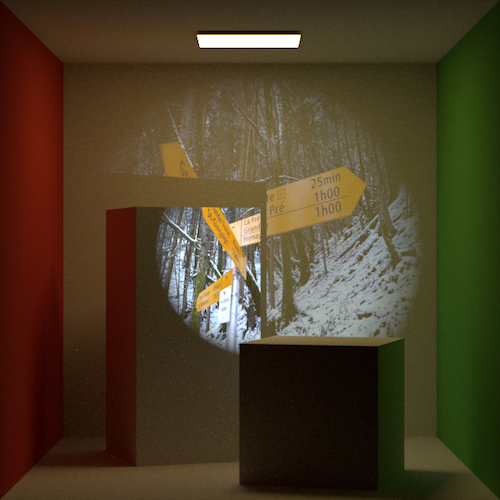
\includegraphics[width=\textwidth]{images/03-projector_features-spotlight.jpg}
        \caption{}
        \label{fig:methods_projector_features_spotlight}
    \end{subfigure}
    \hfill
    \begin{subfigure}[b]{0.32\textwidth}
        \centering
        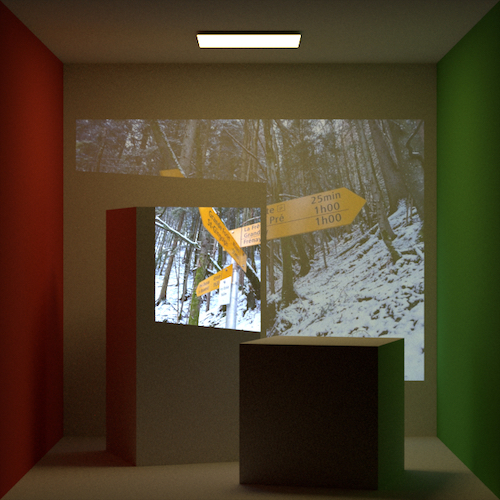
\includegraphics[width=\textwidth]{images/03-projector_features-frustum.jpg}
        \caption{}
        \label{fig:methods_projector_features_frustum}
    \end{subfigure}
    \hfill
    \begin{subfigure}[b]{0.32\textwidth}
        \centering
        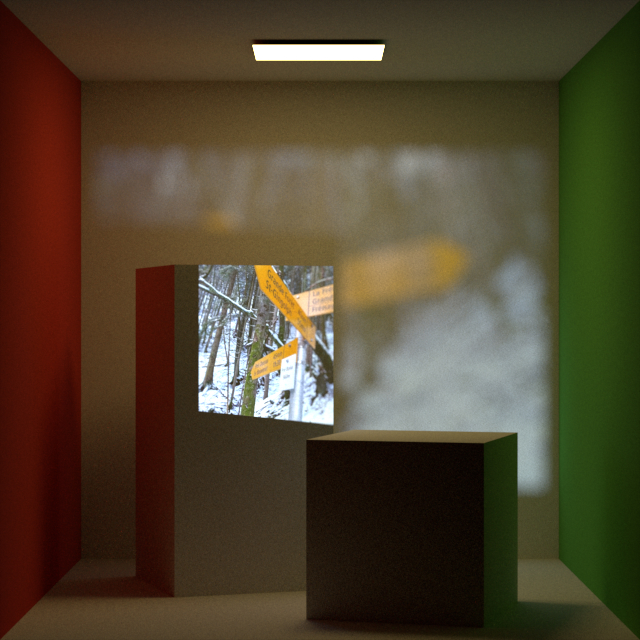
\includegraphics[width=\textwidth]{images/03-projector_features-thin_lens.jpg}
        \caption{}
        \label{fig:methods_projector_features_thin_lens}
    \end{subfigure}
    \caption{Projector features that we have implemented in Mitsuba to support the needs of our projection mapping pipeline. Image \ref{fig:methods_projector_features_spotlight} shows  a spotlight with a projective texture that Mitsuba already supported but was not sufficient for us. Image \ref{fig:methods_projector_features_frustum} shows a rectangular projection frustum that we have added to support rectangular projections. Image \ref{fig:methods_projector_features_thin_lens} shows our final projector implementation with a thin lens optics model that enables the depth of field effect}
    \label{fig:methods_projector_features}
\end{figure}

\textbf{How to solve the rendering equation efficiently with only a single active projector pixel?} Projecting images with our custom projector implementation yields good results (see fig. \ref{fig:methods_projector_features_thin_lens}). However, in order to capture the light transport matrix, we need to project images with only a single active pixel. And this turns out to be problematic due to the way the rendering equation (\ref{eq:rendering_equation}) is typically solved. A \textit{path tracer} (PT), which is the default Monte Carlo solver in Mitsuba and most other renderers, samples random paths from camera, computes radiance travelling along them in the opposite direction and builds an estimate of the final image. In our case, this means that a random walk from the camera needs to sample a single pixel on the projector to yield a light-carrying path. The probability of this happening is extremely low and most paths thus do not contribute anything to the estimate. This results in poor convergence and extremely long rendering time. See fig. \ref{fig:methods_sampling_path} for an example.

However, while some path sampling techniques build path starting from the camera, others start from the emitter. When emitters are very small, like points lights or projectors with only a single white pixel, it is important to start building the path from the light. We therefore use the bi-directional path tracing (BDPT) algorithm which combines paths that start both from the camera and from emitters and which is already implemented in Mitsuba. More on BDPT can be found in \citet{Veach1997}. See fig. \ref{fig:methods_sampling_bdpt} for an example.

Another issue is with sampling a point on the projector where a path could start from. If uniform sampling is used, the only active pixel would be sampled in 1 out of \(m \cdot n\) samples on average where \(m\) and \(n\) are the dimensions of \(p\). This would again yield many paths with zero contribution. To fix this, we have implemented a common variance reduction technique technique used in Monte Carlo integration called \textit{importance sampling}. Importance sampling chooses samples with larger contribution with higher probability. In our case, we base the probability of choosing a projector pixel on the relative contribution of the pixel to the brightness of the whole projector image. This means that when capturing the canonical basis of an LT matrix, the only active pixel is sampled with probability 1 and other pixels are not sampled at all. See fig. \ref{fig:methods_sampling_bdpt_importance} for an example.

\begin{figure}[]
    \centering
    \begin{subfigure}[b]{0.32\textwidth}
        \centering
        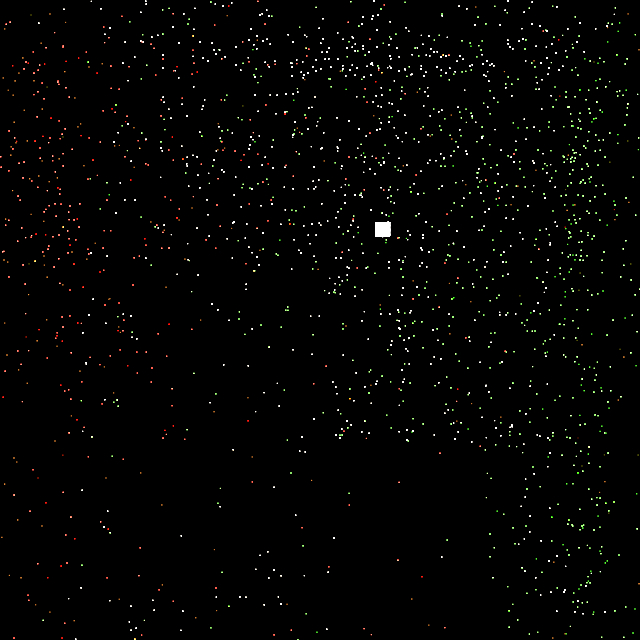
\includegraphics[width=\textwidth]{images/03-sampling_path.jpg}
        \caption{}
        \label{fig:methods_sampling_path}
    \end{subfigure}
    \hfill
    \begin{subfigure}[b]{0.32\textwidth}
        \centering
        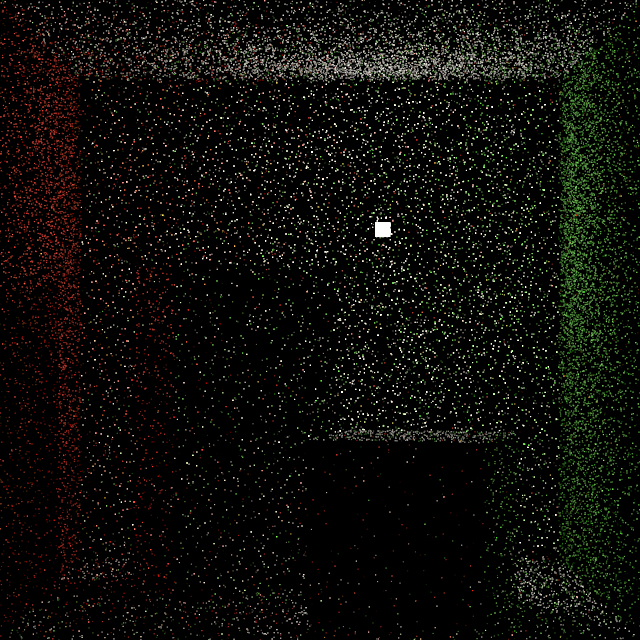
\includegraphics[width=\textwidth]{images/03-sampling_bdpt.jpg}
        \caption{}
        \label{fig:methods_sampling_bdpt}
    \end{subfigure}
    \hfill
    \begin{subfigure}[b]{0.32\textwidth}
        \centering
        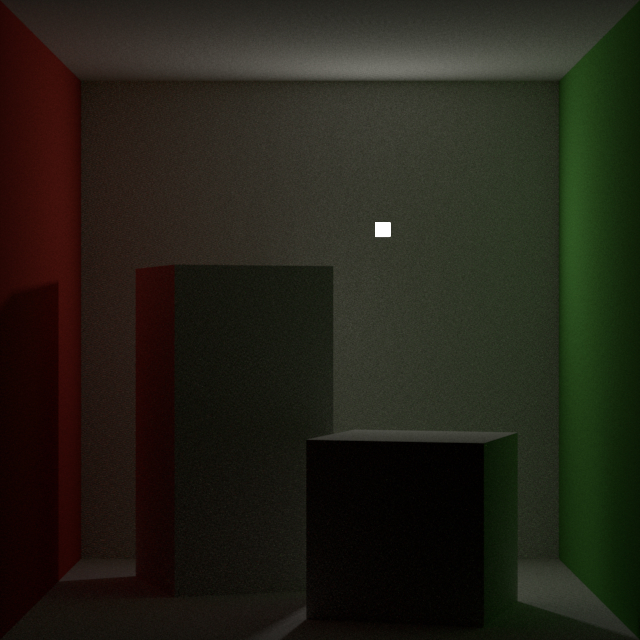
\includegraphics[width=\textwidth]{images/03-sampling_bdpt_importance.jpg}
        \caption{}
        \label{fig:methods_sampling_bdpt_importance}
    \end{subfigure}
    \caption{A comparison of various sampling techniques to solve the rendering equation. The scene is being projected onto by a \(640 \times 480\) image with only a small \(20 \times 20\) patch of active pixels. All images were rendered using 16 path samples per pixel. Image \ref{fig:methods_sampling_path} shows a basic path tracer which samples random light-carrying paths starting from the camera. Image \ref{fig:methods_sampling_bdpt} is bi-directional path tracing (BDPT), a better technique which combines paths from both camera and light sources. Image \ref{fig:methods_sampling_bdpt_importance} shows BDPT with importance sampling of the projector image which greatly reduces noise. This is the method we use in our pipeline}
    \label{fig:methods_sampling}
\end{figure}

\textbf{How large is the light transport matrix and what are the implications?} The last practical consideration we need to make is about the size of the light transport matrix. Here is how it is determined:

\begin{equation}
    \label{eq:lt_matrix_size}
    S = p_w \cdot p_h \cdot c_w \cdot c_h \cdot 3 \cdot 4
\end{equation}

where \(S\) is the matrix size in bytes, \(p_w\) and \(p_h\) is the width and height of the projector image, respectively, \(c_w\) and \(c_h\) are the dimensions of the camera image. We then assume three color channels and four bytes to store each intensity value. It is important to store the intensity values as 32-bit floating point numbers to capture the tiny signal coming from individual projector pixels. See an example of how value precision influences the noise level of basis images in fig. \ref{fig:methods_float}.

This means that an LT matrix for projector and camera image of size \(160 \times 160\) is over 7.8 GB large. This is the size we have used in our experiments because it is sufficient to demonstrate the performance of our method and because it fit well into the memory of our GPUs. However, it is clear that this approach to implementing the rendering function is not very scalable. For our purposes, this approach has the advantage of being simple and accurate which is important when evaluating the basic functionality of a new method. For practical use, more data-efficient methods like those mentioned in section \ref{section:background-projection_mapping-procams-inverse_lt} are needed.

\begin{figure}[]
    \centering
    \begin{subfigure}[b]{0.48\textwidth}
        \centering
        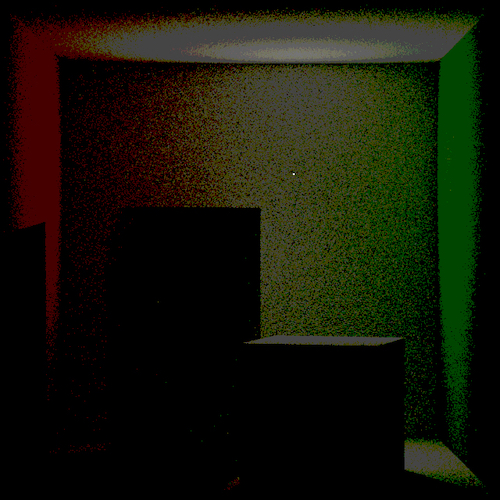
\includegraphics[width=\textwidth]{images/03-floating_point16.jpg}
        \caption{}
        \label{fig:methods_float16}
    \end{subfigure}
    \hfill
    \begin{subfigure}[b]{0.48\textwidth}
        \centering
        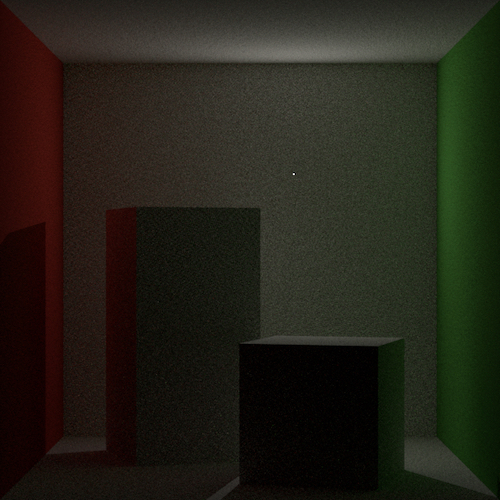
\includegraphics[width=\textwidth]{images/03-floating_point32.jpg}
        \caption{}
        \label{fig:methods_float32}
    \end{subfigure}
    \caption{An illustration of how pixel value precision influences noise level in basis images. The scene is illuminated by a \(640 \times 480\) image where only a single pixel is active. The resulting images are scaled by \(1000000\) for visualization purposes. Image \ref{fig:methods_float16} is stored in 16-bit floating point, while image \ref{fig:methods_float32} is stored in 32-bit floating point}
    \label{fig:methods_float}
\end{figure}

This concludes the section on our rendering function \(x\). In the following section we cover the second building block of our projection mapping pipeline, the texture model \(f\).

\section{Texture Model}
\label{section:methods-texture_model}

Our texture model is built on top of that used in \citet{Gatys2015} and described in section \ref{section:background-texture_synthesis-statistics_based-synthesis_using_cnns}. While the vanilla Gatys model achieves very good results, it also has several shortcomings, such as desaturated patches when synthesizing textures larger than input or physically implausible feature deformation (see figs. \ref{fig:methods_comparison_small-vanilla} and \ref{fig:methods_comparison_large-vanilla} for examples).

These shortcomings are well known and have been studied by several authors who have introduced improvements to the original model which result in higher quality texture synthesis. It is unclear, however, whether improvements in texture synthesis also translate into improvements in the projection mapping of textures. We have thus decided to reimplement the original Gatys model along with the improvements and evaluate how each of them peforms in our setup.

\citet{Gatys2015} have provided an implementation of their algorithm in the Caffe (\citet{Jia2014}) deep learning framework. Because this framework is not very commonly used anymore (last stable version was released in 2017, according to \citet{CaffeGitHub}), we have ported the algorithm to PyTorch which is currently more actively maintained and therefore easier to work with.

\subsection{Improving Gatys Texture Synthesis}
\label{section:methods-texture_model-improvements}

As discussed in section \ref{section:background-texture_synthesis-statistics_based-synthesis_using_cnns}, the original Gatys algorithm synthesizes a texture \(y_2\) from an example \(y_1\) by minimizing the difference between their statistics \(f(y_2)\) and \(f(y_1)\) which fully describe a texture under the Gatys texture model. The specific form of \(f\) determines the performance of the synthesis algorithm.

We have implemented three different improvements to the original Gatys statistics. In general, all of them tend to reduce the ambiguity of the texture description (i.e. reduce the size of texture classes as defined by their texture model) and thus better enforce texture structure while maintaining high variance of reasonable outputs. We now briefly describe each of the three improvements.

\subsubsection{Activation Shift}
\label{section:methods-texture_model-improvements-activation_shift}

In the original Gatys model, a set Gram matrices of VGG-19 layer activations form the set of descriptive statistics \(f\):

\begin{equation}
    \label{eq:gatys_statistics}
    f(y) = \{G^1(y), \dots, G^L(y)\}
\end{equation}

where \(L\) is a chosen number of VGG-19 layers that are used for synthesis and a Gram matrix \(G^l(y)\) is defined as

\begin{equation}
    \label{eq:gram_style}
    G_{ij}^l(y) = \sum_k F_{ik}^l(y) F_{jk}^l(y)
\end{equation}

where \(i\) and \(j\) are filters in layer \(l\) and \(F_{jk}^l\) is the activation of the \(j\)-th filter at position \(k\) in layer \(l\). A Gram matrix thus represents the correlations between feature reponses in a network layer.

\citet{Novak2016} have introduced a number of simple improvements to the way Gram matrices are calculated from VGG-19 activations. One of them is called \textit{activation shift}. In the original Gatys model, activations \(F_{jk}^l\) are non-negative with mean 1. Also, the resulting Gram matrices \(G^l\) tend to be very sparse with many zero entries. \citet{Novak2016} argue that these zero entries are a source of ambiguity in texture description because they could have many causes:

\begin{itemize}
    \item Both features that the activations represent are missing from the image
    \item Only one of the features is present
    \item Both of them are present but never appear together
\end{itemize}

To remove this ambiguity, \citet{Novak2016} suggest to offset the activations by \(-1\) before computing the Gram matrices:

\begin{equation}
    \label{eq:gram_style_activation_shift}
    G_{ij}^l = \sum_k (F_{ik}^l - 1) (F_{jk}^l - 1)
\end{equation}

This is extremely simple to implement and brings clear improvements to synthesis quality (see figs. \ref{fig:methods_comparison_small-shift} and \ref{fig:methods_comparison_large-shift}).

\subsubsection{Correlation Chain}
\label{section:methods-texture_model-improvements-correlation_chain}

\citet{Novak2016} present one more useful modification to Gram matrix computation. In the original algorithm, only activations from the same layer are correlated with each other to form a Gram matrix. \citet{Novak2016} suggest to correlate activations from neighbouring layers as well. Because activation maps \(F^l\) and \(F^k\) where \(l\) and \(k\) are neighbouring layers may have different dimensions, the smaller map needs to be upsampled first. As a result a new set of matrices \(G^{lk}\) is added to the original set \(G^l\) to further lower the ambiguity of the texture description:

\begin{equation}
    \label{eq:gram_style_chain}
    G^{lk} = F^l [\textit{up}(F^k)]^T
\end{equation}

where \(l = 1 \dots L - 1\), \(L\) is the number of chosen layers, \(k = l + 1\) and \textit{up} is an upsampling procedure. The contribution of this modification to texture synthesis can be seen in figs. \ref{fig:methods_comparison_small-chain} and \ref{fig:methods_comparison_large-chain}.

\subsubsection{Gaussian Pyramid}
\label{section:methods-texture_model-improvements-gaussian_pyramid}

\citet{Snelgrove2017} has observed that the performance of Gatys synthesis is greatly limited by the receptive fields of the underlying VGG-19 network. The network was trained on images of size \(224 \times 224\) and its capability to capture information about large features is larger images is thus limited (see \ref{fig:methods_receptive_field} for an illustration).

\begin{figure}[]
    \centering
    \begin{subfigure}[b]{0.48\textwidth}
        \centering
        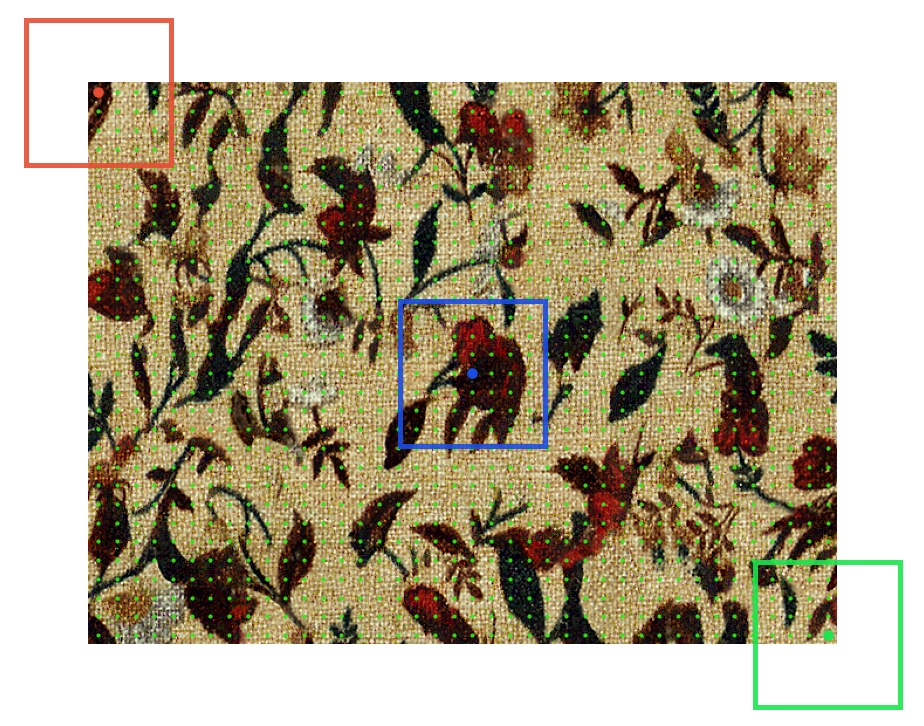
\includegraphics[width=\textwidth]{images/03-receptive_field-level0.jpg}
        \caption{}
        \label{fig:methods_receptive_field_lvl0}
    \end{subfigure}
    \hfill
    \begin{subfigure}[b]{0.48\textwidth}
        \centering
        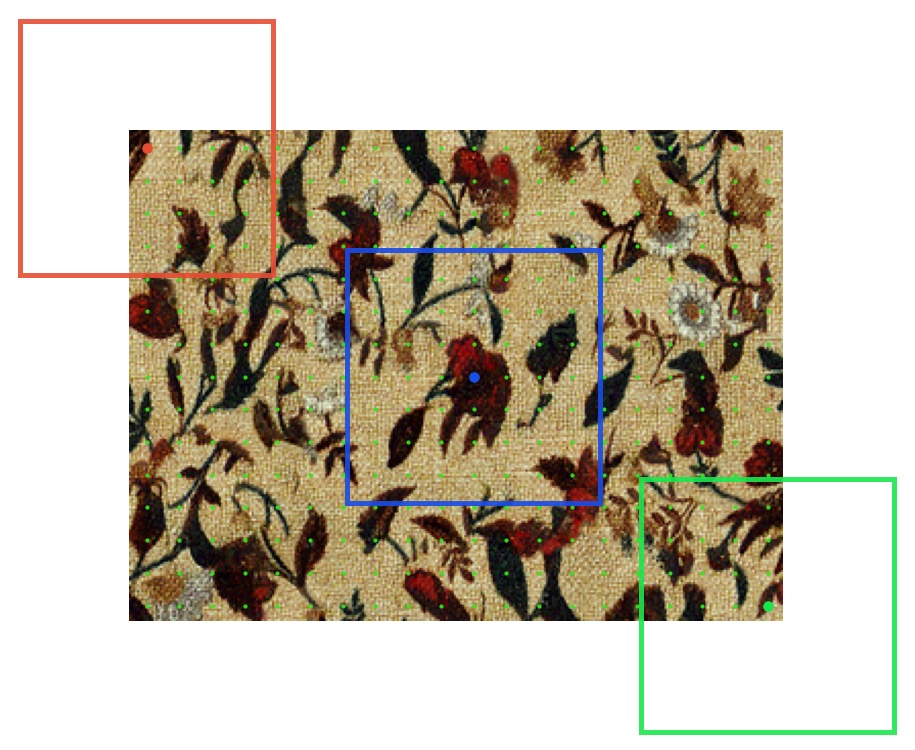
\includegraphics[width=\textwidth]{images/03-receptive_field-level1.jpg}
        \caption{}
        \label{fig:methods_receptive_field_lvl1}
    \end{subfigure}
    \caption{A comparison of the receptive fields of the last layer of VGG-19 used in the Gatys texture model. A receptive field of a network layer activation is essentially a patch of pixels of the input image which has an effect on that particular activation. If a texture feature is larger than the receptive field of a given activation, then it cannot be captured by statistics computed on the activation. Figure \ref{fig:methods_receptive_field_lvl0} uses an input image of size \(640 \times 480\) while figure \ref{fig:methods_receptive_field_lvl1} uses size \(320 \times 240\). Texture source: \citet{Pixar128}}
    \label{fig:methods_receptive_field}
\end{figure}

To fix this, he proposes to not compute the Gram matrices on images, but rather on Gaussian pyramids of images. This means that instead of eq. \ref{eq:gatys_statistics}, he uses

\begin{equation}
    \label{eq:snelgrove_statistics}
    f(y) = \{\{G^1(y_i) | i = 1, \dots, s\}, \dots, \{G^L(y_i) | i = 1, \dots, s\}\}
\end{equation}

where \(y_i\) is image \(y_{i - 1}\) downsampled by half using proper pre-filtering, such as Lanczos. \(s\) is a chosen number of scales which depends on the size of the texture we wish to synthesize. As a result, even more Gram matrices are used to further disambiguate the texture description. Results of this modification can be seen in figs. \ref{fig:methods_comparison_small-pyramid} and \ref{fig:methods_comparison_large-pyramid}.

\begin{figure}[ht]
    \centering    
    \begin{subfigure}{0.8\textwidth}
        \centering
        \begin{subfigure}{0.32\textwidth}
            \centering
            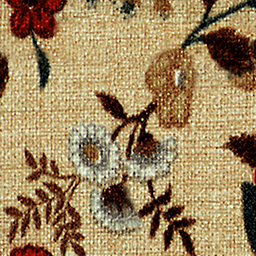
\includegraphics[width=\textwidth]{images/03-comparison_small_target.jpg}
            \caption{Input}
            \label{fig:methods_comparison_small-target}
        \end{subfigure}
        \hfill
        \begin{subfigure}{0.32\textwidth}
            \centering
            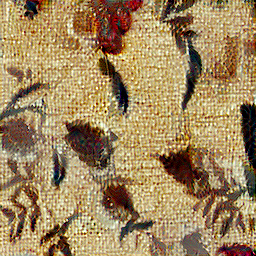
\includegraphics[width=\textwidth]{images/03-comparison_small_vanilla.jpg}
            \caption{Gatys}
            \label{fig:methods_comparison_small-vanilla}
        \end{subfigure}
        \hfill
        \begin{subfigure}{0.32\textwidth}
            \centering
            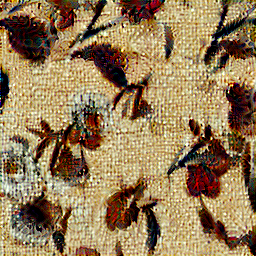
\includegraphics[width=\textwidth]{images/03-comparison_small_shift.jpg}
            \caption{Shift}
            \label{fig:methods_comparison_small-shift}
        \end{subfigure}
        
        \begin{subfigure}{0.32\textwidth}
            \centering
            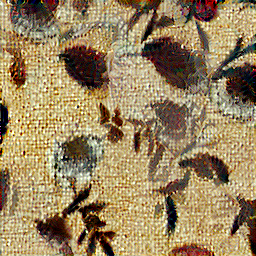
\includegraphics[width=\textwidth]{images/03-comparison_small_chain.jpg}
            \caption{Chain}
            \label{fig:methods_comparison_small-chain}
        \end{subfigure}
        \hfill
        \begin{subfigure}{0.32\textwidth}
            \centering
            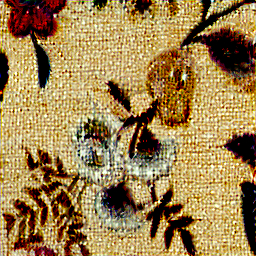
\includegraphics[width=\textwidth]{images/03-comparison_small_pyramid.jpg}
            \caption{Pyramid}
            \label{fig:methods_comparison_small-pyramid}
        \end{subfigure}
        \hfill
        \begin{subfigure}{0.32\textwidth}
            \centering
            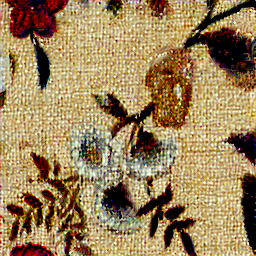
\includegraphics[width=\textwidth]{images/03-comparison_small_pyramid_shift.jpg}
            \caption{Pyramid + Shift}
            \label{fig:methods_comparison_small-pyramid_shift}
        \end{subfigure}
        \vskip 20pt
        % -------------------------------------------
        \begin{subfigure}{0.32\textwidth}
            \centering
            
\includegraphics[width=\textwidth]{images/03-comparison_large_target.jpg}
            \caption{Input}
            \label{fig:methods_comparison_large-target}
        \end{subfigure}
        \hfill
        \begin{subfigure}{0.32\textwidth}
            \centering
            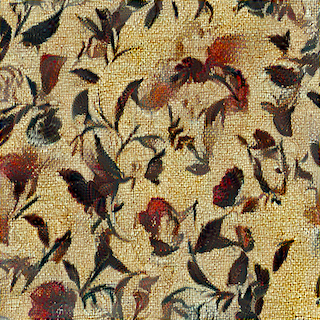
\includegraphics[width=\textwidth]{images/03-comparison_large_vanilla.jpg}
            \caption{Gatys}
            \label{fig:methods_comparison_large-vanilla}
        \end{subfigure}
        \hfill
        \begin{subfigure}{0.32\textwidth}
            \centering
            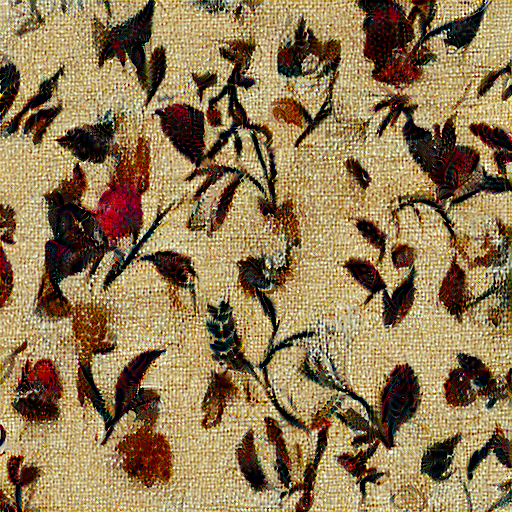
\includegraphics[width=\textwidth]{images/03-comparison_large_shift.jpg}
            \caption{Shift}
            \label{fig:methods_comparison_large-shift}
        \end{subfigure}
        
        \begin{subfigure}{0.32\textwidth}
            \centering
            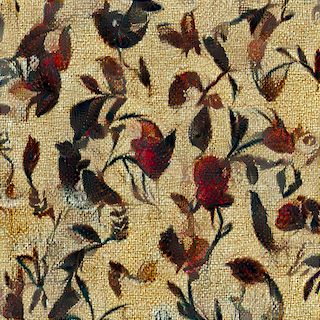
\includegraphics[width=\textwidth]{images/03-comparison_large_chain.jpg}
            \caption{Chain}
            \label{fig:methods_comparison_large-chain}
        \end{subfigure}
        \hfill
        \begin{subfigure}{0.32\textwidth}
            \centering
            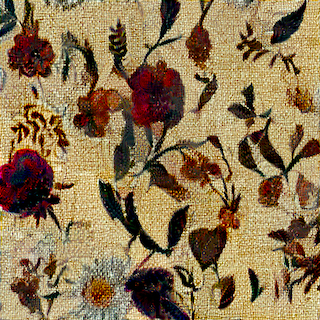
\includegraphics[width=\textwidth]{images/03-comparison_large_pyramid.jpg}
            \caption{Pyramid}
            \label{fig:methods_comparison_large-pyramid}
        \end{subfigure}
        \hfill
        \begin{subfigure}{0.32\textwidth}
            \centering
            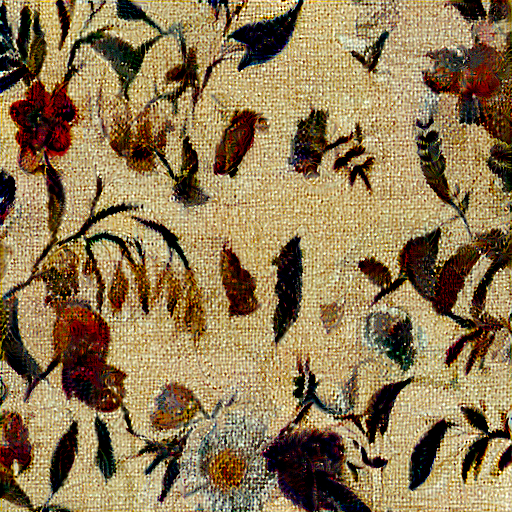
\includegraphics[width=\textwidth]{images/03-comparison_large_pyramid_shift.jpg}
            \caption{Pyramid + Shift}
            \label{fig:methods_comparison_large-pyramid_shift}
        \end{subfigure}
    \end{subfigure}
    \caption{A comparison of synthesis under various texture models described in this section. The upper two rows contain images of size \(256 \times 256\) while the lower two rows contain images of size \(512 \times 512\). Note desaturated patches and inaccurate colors when Shift is not used and large feature distortion under the Gatys texture model. Lastly, note that Pyramid describes the small texture so accurately that it synthesizes an image identical to the input. Texture source: \citet{Pixar128}}
    \label{fig:methods_comparison_small}
\end{figure}

{\color{red} TODO: explain also how you optimize and parameterize (Jaakko thinks that I'm using a sigmoid to restrict pixel values between 0 and 1\dots)}